\documentclass[11pt,a4paper]{article}

\usepackage[utf8]{inputenc}
\usepackage[T1]{fontenc}
\usepackage[margin=2.5cm]{geometry}
\setlength{\headheight}{14pt}
\usepackage[colorlinks=true,linkcolor=red!60!black,urlcolor=blue!60!black,citecolor=blue!60!black]{hyperref}
\usepackage{xcolor}
\usepackage{booktabs}
\usepackage{listings}
\usepackage{enumitem}
\usepackage{titlesec}
\usepackage{parskip}
\usepackage{microtype}
\usepackage{fancyhdr}
\usepackage{tabularx}
\usepackage{tikz}
\usetikzlibrary{positioning, arrows.meta, fit, backgrounds, shapes.geometric}

\definecolor{usydred}{HTML}{C63B1E}
\definecolor{ochre}{HTML}{C4972A}
\definecolor{sandstone}{HTML}{E8D5B5}
\definecolor{charcoal}{HTML}{2D2926}
\definecolor{eucalypt}{HTML}{567D46}
\definecolor{codebg}{HTML}{F5F0E8}
\definecolor{mutedtext}{HTML}{6B6560}

\titleformat{\section}{\Large\bfseries\color{usydred}}{\thesection}{1em}{}
\titleformat{\subsection}{\large\bfseries\color{charcoal}}{\thesubsection}{1em}{}
\titleformat{\subsubsection}{\normalsize\bfseries\color{charcoal}}{\thesubsubsection}{1em}{}

\lstdefinestyle{code}{
  basicstyle=\ttfamily\small,
  backgroundcolor=\color{codebg},
  frame=single,
  framesep=6pt,
  rulecolor=\color{sandstone},
  breaklines=true,
  keywordstyle=\color{usydred},
  commentstyle=\color{mutedtext}\itshape,
  stringstyle=\color{ochre},
  numbers=none,
  showstringspaces=false,
  upquote=true,
}
\lstset{style=code}

\lstdefinestyle{shell}{
  style=code,
  basicstyle=\ttfamily\footnotesize,
}

\pagestyle{fancy}
\fancyhf{}
\fancyhead[L]{\textcolor{mutedtext}{\small DASH Repository: Setup and Operations Walkthrough}}
\fancyhead[R]{\textcolor{mutedtext}{\small \thepage}}
\renewcommand{\headrulewidth}{0pt}

\title{\vspace{-2cm}\textcolor{usydred}{\rule{\textwidth}{4pt}}\\[1em]
\Huge\bfseries Setting up and running the\\DASH Repository mockup\\[0.4em]
\large\mdseries\color{mutedtext} How everything is wired, how to operate it, and how to move it}
\author{\small Charles Perkins Centre, Data Science Hub \\ \small University of Sydney}
\date{June 2026}

\begin{document}
\maketitle
\thispagestyle{empty}

\begin{quote}
\itshape\color{mutedtext}\small
This document is the operating manual for the DASH Repository mockup as it exists at the end of Phase 1's build phase. It assumes you can navigate a terminal and have basic familiarity with git, but it does not assume prior knowledge of Cloudflare Workers, MongoDB Atlas, or any of the specific services involved. The aim is that whoever picks this up next, you or someone else, can get from a fresh laptop to a working deployment without needing to ask.
\end{quote}

\vspace{1em}
\tableofcontents
\vspace{2em}

\section{What this document is}

This document describes a working mockup of the DASH Repository: a search system that lets researchers ask natural-language questions about past DASH consultations and get back the most relevant past projects. The mockup is live at the time of writing, with a frontend, an API server, a database, and a CI/CD pipeline all wired together.

You should read this document if you need to:

\begin{itemize}[leftmargin=1.5em,itemsep=2pt]
  \item Understand how the system is put together (Section 2).
  \item Set the whole thing up from scratch on a new set of accounts (Sections 3 to 6).
  \item Add a new project to the catalogue, or edit the code (Section 7).
  \item Move the mockup off your personal Cloudflare or Atlas accounts onto DASH-owned infrastructure (Section 8).
  \item Figure out why something has stopped working (Section 9).
  \item Look up where a specific file lives or which environment variable controls what (Section 10).
\end{itemize}

The document is written so it can be read top to bottom on a first pass, then used as a reference afterwards. If you only have time to read one section, read Section 2.

\section{The system at a glance}

The mockup has six pieces working together. Five of them are services run by other people that we pay for or use for free; the sixth is a stateless server we operate ourselves.

\subsection{The six pieces}

\begin{center}
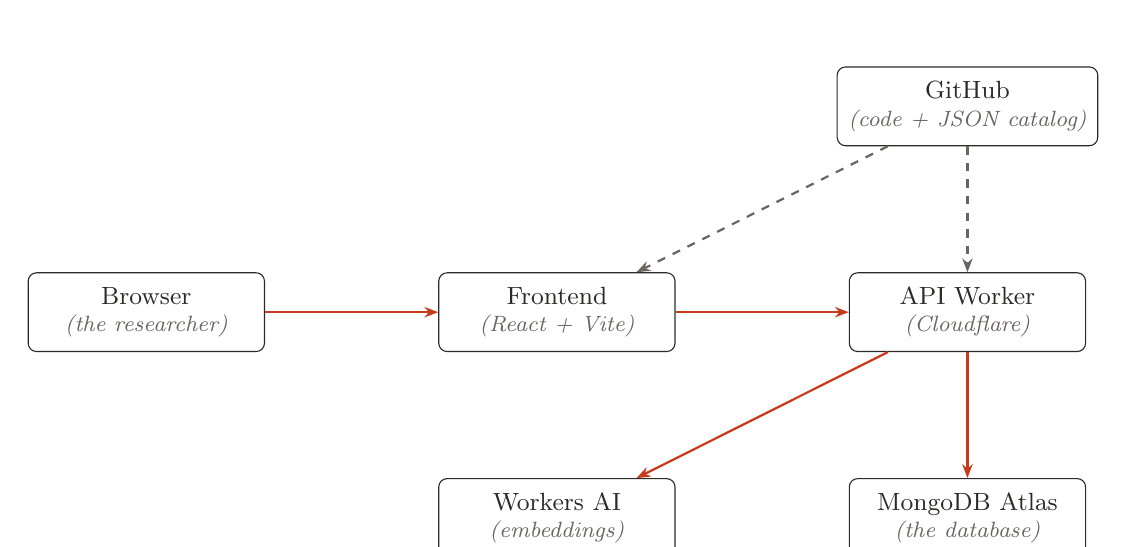
\begin{tikzpicture}[
  every node/.style={font=\small, text=charcoal},
  component/.style={
    draw=charcoal,
    rounded corners=3pt,
    minimum width=3.0cm,
    minimum height=1.0cm,
    fill=white,
    align=center,
    inner sep=4pt,
  },
  loclabel/.style={
    font=\small\itshape,
    text=mutedtext,
  },
  link/.style={
    -{Stealth[length=5pt]},
    thick,
    draw=usydred,
  },
  arrowlabel/.style={
    font=\scriptsize,
    text=charcoal,
    inner sep=2pt,
    fill=white,
  },
]
  \node[component] (browser) {Browser \\[-1pt] {\footnotesize\itshape\color{mutedtext}(the researcher)}};
  \node[component, right=2.2cm of browser] (frontend) {Frontend \\[-1pt] {\footnotesize\itshape\color{mutedtext}(React + Vite)}};
  \node[component, right=2.2cm of frontend] (api) {API Worker \\[-1pt] {\footnotesize\itshape\color{mutedtext}(Cloudflare)}};
  \node[component, below=1.6cm of frontend] (ai) {Workers AI \\[-1pt] {\footnotesize\itshape\color{mutedtext}(embeddings)}};
  \node[component, below=1.6cm of api] (atlas) {MongoDB Atlas \\[-1pt] {\footnotesize\itshape\color{mutedtext}(the database)}};
  \node[component, above=1.6cm of api] (github) {GitHub \\[-1pt] {\footnotesize\itshape\color{mutedtext}(code + JSON catalog)}};

  \draw[link] (browser) -- (frontend);
  \draw[link] (frontend) -- (api);
  \draw[link] (api) -- (ai);
  \draw[link] (api) -- (atlas);
  \draw[link, dashed, draw=mutedtext] (github) -- (api);
  \draw[link, dashed, draw=mutedtext] (github) -- (frontend);
\end{tikzpicture}
\end{center}

\smallskip
\noindent{\small\itshape\color{mutedtext} Solid arrows show the live request path during a search. Dashed arrows show the deploy path: GitHub Actions ships code changes to the Worker and the frontend.}

\medskip

The six pieces and what each one does:

\begin{enumerate}[leftmargin=1.5em,itemsep=4pt]
  \item \textbf{Browser.} What the researcher uses. They open a URL, they type a question, they see results. We do not operate this; the user's own laptop runs it.
  \item \textbf{Frontend.} A small static web app written in React with Vite as the build tool. It is the page the researcher actually sees. It calls the API for results and renders them. It is hosted on Cloudflare and served from \texttt{https://dash-frontend.<subdomain>.workers.dev}.
  \item \textbf{API Worker.} A small server written in JavaScript that runs on Cloudflare's edge network. It exposes a few HTTP endpoints. It takes a query from the frontend, asks Workers AI to turn it into a vector, asks MongoDB Atlas to find the closest matching projects, and returns the results. It is hosted on Cloudflare at \texttt{https://dash-api.<subdomain>.workers.dev}.
  \item \textbf{Workers AI.} Cloudflare's embedding service. We send it a piece of text, it sends back a list of 1024 numbers (a vector) that represents the meaning of the text. We use the model \texttt{bge-large-en-v1.5}. We do not operate this.
  \item \textbf{MongoDB Atlas.} The database. It holds one document per project, including the metadata, the executive summary, and the embedding vector. It also performs the vector similarity search at query time. We do not operate the database itself, but we own the data and the schema.
  \item \textbf{GitHub.} Where the code lives and where new project metadata is added. Pushing to GitHub triggers GitHub Actions, which redeploys the API Worker (if the API code changed) or pushes new project metadata into MongoDB (if a project JSON changed).
\end{enumerate}

\subsection{What happens on a single search}

Walking through a query from end to end:

\begin{enumerate}[leftmargin=1.5em,itemsep=2pt]
  \item The researcher opens the frontend URL in their browser. The frontend's JavaScript loads, the page renders.
  \item The researcher types ``find proteomics work on inflammatory skin conditions'' and submits.
  \item The frontend POSTs the query as JSON to \texttt{https://dash-api.<sub>.workers.dev/api/ask}.
  \item The API Worker receives the request. It calls Cloudflare's Workers AI with the query text. Workers AI returns a 1024-element vector.
  \item The API Worker sends a query to MongoDB Atlas asking for the projects whose stored vectors are closest to the query vector. Atlas returns the top matches with a similarity score.
  \item The API Worker formats the results, builds a short prose answer (``I found 3 DASH projects related to \ldots''), and returns JSON to the frontend.
  \item The frontend renders the answer as a chat message and the matches as cards. The researcher clicks a card to read more, which opens a side drawer with the full project details.
\end{enumerate}

End to end, this takes roughly 300 to 400 milliseconds: about 200 ms for the embedding call, 50 ms for the database query, and the rest in network round trips.

\section{Initial setup: the accounts and credentials}

Setting up the mockup from scratch takes about an hour if you have credentials for the three external services. Most of the work is clicking through web dashboards. The actual code does not need to be modified at any point during initial setup.

You will need to set up, in order:

\begin{enumerate}[leftmargin=1.5em,itemsep=2pt]
  \item A Cloudflare account
  \item A MongoDB Atlas account
  \item A GitHub account, with a copy of the repository
  \item A handful of secrets and tokens linking the three together
\end{enumerate}

\subsection{Cloudflare account}

Sign up at \href{https://dash.cloudflare.com/sign-up}{dash.cloudflare.com/sign-up}. The free plan covers everything the mockup uses: Workers, Workers AI, and DNS.

Once you are signed in:

\begin{enumerate}[leftmargin=1.5em,itemsep=2pt]
  \item Note your \textbf{Account ID}, shown on the right sidebar of the Workers \& Pages page. You will need this later.
  \item Confirm you have access to \textbf{Workers AI} by visiting Workers \& Pages \(\rightarrow\) AI. New Cloudflare accounts have this enabled by default.
  \item Pick a \textbf{workers.dev subdomain}. When you deploy your first Worker, Cloudflare prompts you to pick one. Choose something memorable; you cannot easily change it.
\end{enumerate}

\subsection{MongoDB Atlas account and cluster}

Sign up at \href{https://www.mongodb.com/cloud/atlas/register}{mongodb.com/cloud/atlas/register}. Once in:

\begin{enumerate}[leftmargin=1.5em,itemsep=2pt]
  \item Create a new \textbf{Atlas Flex cluster}. Region: AWS Sydney (\texttt{ap-southeast-2}). Cluster name: anything; \texttt{dash} is fine. Atlas Flex costs about \$8 per month at our usage; the M0 free tier is not recommended for vector search.
  \item Create a \textbf{database user} with read/write access to your \texttt{dash} database. Save the username and password.
  \item Set \textbf{network access} to allow \texttt{0.0.0.0/0} (anywhere). This is mockup-acceptable because the connection is gated by username/password. Production should restrict to Cloudflare's egress IPs.
  \item Note the cluster's \textbf{connection string} from the \texttt{Connect} dialog. It looks like:
\begin{lstlisting}[style=shell]
mongodb+srv://<user>:<password>@dash.xxxxx.mongodb.net/?retryWrites=true&w=majority
\end{lstlisting}
  Replace \verb|<user>| and \verb|<password>| with the actual credentials. This whole string is what we call \texttt{ATLAS\_URI}.
\end{enumerate}

\subsection{Apply the Atlas indexes}

The mockup expects three indexes on the \texttt{dash.projects} collection. Apply them via the Atlas dashboard \(\rightarrow\) your cluster \(\rightarrow\) Collections \(\rightarrow\) Atlas Search and Indexes tabs:

\begin{enumerate}[leftmargin=1.5em,itemsep=2pt]
  \item \textbf{Vector search index} (\texttt{projects\_vector}): paste the JSON from \texttt{option\_b/atlas/vector-index.json} in the repo. This is the index that powers natural-language search.
  \item \textbf{Compound indexes}: same idea, the JSON in \texttt{option\_b/atlas/compound-indexes.json}.
  \item \textbf{Text search index} (\texttt{projects\_text}): the JSON in \texttt{option\_b/atlas/search-indexes.json}.
\end{enumerate}

Each index takes a couple of minutes to build the first time. They self-maintain after that.

\subsection{GitHub repository}

If you are setting this up from scratch:

\begin{enumerate}[leftmargin=1.5em,itemsep=2pt]
  \item Clone the existing repo locally:
\begin{lstlisting}[style=shell]
git clone https://github.com/ecool50/dash-repo-prototype.git
cd dash-repo-prototype
\end{lstlisting}
  \item Either fork it to your own GitHub account, or transfer ownership to whichever organisation you want to host it under. We will refer to the new owner as \texttt{<org>} from here.
\end{enumerate}

\subsection{Generate the ingest secret}

The CI/CD pipeline that pushes new projects into MongoDB calls a protected endpoint on the API Worker. The endpoint checks an \texttt{Authorization: Bearer ...} header. The token is something you generate yourself:

\begin{lstlisting}[style=shell]
openssl rand -hex 32
\end{lstlisting}

This prints a 64-character random string. Save it somewhere safe (a password manager). The same value goes in two places, the Cloudflare Worker (as a secret) and GitHub Actions (as a secret).

\subsection{Summary of what you should now have}

Before continuing to deployment, you should have collected:

\begin{itemize}[leftmargin=1.5em,itemsep=2pt]
  \item A Cloudflare account, account ID noted
  \item A MongoDB Atlas cluster in Sydney, three indexes applied
  \item A MongoDB connection string (the \texttt{ATLAS\_URI})
  \item A copy of the repository under your control
  \item A 64-character random hex string (the ingest secret)
\end{itemize}

You will also need, but can get later:

\begin{itemize}[leftmargin=1.5em,itemsep=2pt]
  \item A \textbf{Cloudflare API token} with Workers Edit permission, for GitHub Actions to deploy on your behalf. We will create this in Section 6.
  \item The \textbf{deployed Worker URL}, for the frontend and for GitHub Actions to know where to send ingest requests. We will get this in Section 4.
\end{itemize}

\section{Deploying the API Worker}

The API Worker is the heart of the system: it serves the search endpoint that the frontend calls. Deploying it from a fresh laptop takes about ten minutes.

\subsection{Install Wrangler}

Wrangler is Cloudflare's command-line tool for managing Workers. The repo's \texttt{option\_b/package.json} already pins a compatible version, so we install via npm:

\begin{lstlisting}[style=shell]
cd option_b
npm install
\end{lstlisting}

This installs Wrangler and the MongoDB driver into \texttt{option\_b/node\_modules}.

\subsection{Authenticate Wrangler with your Cloudflare account}

\begin{lstlisting}[style=shell]
cd option_b/api
npx wrangler login
\end{lstlisting}

This opens a browser, asks you to authorize Wrangler against your Cloudflare account, and stores credentials locally. You only have to do this once per machine.

\subsection{Set the Worker secrets}

The Worker needs two secret values: the MongoDB connection string and the ingest secret. Set them with Wrangler:

\begin{lstlisting}[style=shell]
npx wrangler secret put ATLAS_URI
# Paste the full mongodb+srv://... string when prompted, press Enter.

npx wrangler secret put INGEST_SECRET
# Paste the 64-character random string from openssl, press Enter.
\end{lstlisting}

Both values are now stored encrypted on Cloudflare's side and made available to the Worker at runtime as \texttt{env.ATLAS\_URI} and \texttt{env.INGEST\_SECRET}. You cannot read them back; if you forget the value, you set a new one.

You can confirm both are present (without seeing the values) with:

\begin{lstlisting}[style=shell]
npx wrangler secret list
\end{lstlisting}

The output should list \texttt{ATLAS\_URI} and \texttt{INGEST\_SECRET}.

\subsection{Deploy the Worker}

\begin{lstlisting}[style=shell]
npx wrangler deploy
\end{lstlisting}

Wrangler bundles the code in \texttt{option\_b/api/}, uploads it, and prints the deployed URL. On a fresh account this is the moment Cloudflare asks you to pick a workers.dev subdomain. After that, you see:

\begin{lstlisting}[style=shell]
Uploaded dash-api (X.XX sec)
Published dash-api
  https://dash-api.<your-subdomain>.workers.dev
\end{lstlisting}

That URL is now your live API. Save it; you will need it twice more during setup (once for the frontend's \texttt{.env.production}, once for a GitHub Actions secret).

\subsection{Smoke test the deployed Worker}

The repo includes a smoke test script that hits every endpoint and reports pass or fail:

\begin{lstlisting}[style=shell]
cd ../..  # back to repo root
option_b/scripts/smoke.sh https://dash-api.<your-subdomain>.workers.dev
\end{lstlisting}

You should see PASS on six checks. If the database is empty (which it will be on a fresh Atlas cluster), the search endpoint will return zero results but still succeed; that's fine.

If anything fails here, see Section 9 on troubleshooting before continuing.

\subsection{Load initial project data}

If you want to load the ten illustrative projects right now, from the repo root:

\begin{lstlisting}[style=shell]
ATLAS_URI='<your-mongodb-connection-string>' \
  node option_b/scripts/ingest.mjs option_b/projects/A*.json
\end{lstlisting}

This ingests each JSON in turn. The script is idempotent: running it twice has the same effect as running it once. After this, the smoke test's search check should return actual matches.

\section{Deploying the frontend}

The frontend is a small React app built with Vite. It lives in \texttt{dash\_frontend/} at the repo root. Deploying it to Cloudflare also takes about ten minutes.

\subsection{Wire the frontend to the API}

The frontend reads the API URL from an environment variable at build time. The file \texttt{dash\_frontend/.env.production} sets this:

\begin{lstlisting}[style=code]
VITE_API_BASE_URL=https://dash-api.<your-subdomain>.workers.dev
\end{lstlisting}

If you are deploying on a different Cloudflare account than the one the repo was originally set up for, update this file with your own Worker URL before deploying.

\subsection{Build and deploy the frontend Worker}

The frontend is deployed as a Cloudflare Worker with an assets binding, which means the Worker serves the built static files. The configuration lives in \texttt{dash\_frontend/wrangler.toml}. To deploy manually:

\begin{lstlisting}[style=shell]
cd dash_frontend
npm install
npm run build
npx wrangler deploy
\end{lstlisting}

This builds the Vite bundle into \texttt{dash\_frontend/dist/}, then uploads it as a Worker. The output prints the frontend URL:

\begin{lstlisting}[style=shell]
Deployed dash-frontend triggers
  https://dash-frontend.<your-subdomain>.workers.dev
\end{lstlisting}

Open that URL in a browser. You should see the DASH chat interface with a starter message and suggested queries.

\subsection{Test a query end to end}

Click one of the suggested queries, for example ``find proteomics work on inflammatory skin conditions''. You should see a loading spinner, then a short agent message, then a grid of result cards. If you have loaded the ten illustrative projects, the top result is \texttt{A01: Proteomic profiling of a chronic inflammatory skin condition}.

Click ``Open Details'' on a card to see the side drawer with the full project description.

\subsection{Setting up the deploy via Cloudflare's dashboard}

The above is the manual one-off deploy. To make subsequent deploys automatic (every push to GitHub redeploys the frontend), connect the frontend to GitHub via the Cloudflare dashboard:

\begin{enumerate}[leftmargin=1.5em,itemsep=2pt]
  \item Cloudflare \(\rightarrow\) Workers \& Pages \(\rightarrow\) Create application \(\rightarrow\) Connect to Git.
  \item Pick your repository.
  \item Project name: \texttt{dash-frontend}.
  \item Root directory (sometimes called Path): \texttt{dash\_frontend}.
  \item Build command: \texttt{npm install \&\& npm run build}.
  \item Deploy command: \texttt{npx wrangler deploy}.
  \item Save and deploy.
\end{enumerate}

After this, every git push triggers a fresh build and deploy.

\section{CI/CD: GitHub Actions for the API and the catalog}

The repository has two GitHub Actions workflows that handle continuous deployment for the API Worker and continuous ingestion for new project metadata. Setting these up requires four GitHub secrets.

\subsection{The two workflows in plain language}

\begin{itemize}[leftmargin=1.5em,itemsep=4pt]
  \item \texttt{.github/workflows/deploy-worker.yml}: fires whenever code under \texttt{option\_b/api/} changes on the main branch. It checks out the repo, installs dependencies, and runs \texttt{wrangler deploy}. Result: the API Worker is redeployed within a minute or two of every push that touches the API code.
  \item \texttt{.github/workflows/ingest-catalog.yml}: fires whenever any JSON file under \texttt{option\_b/projects/} changes on main. It diffs the changed files, then POSTs each one to the deployed Worker's \texttt{/api/ingest} endpoint. The Worker validates, embeds, and writes to MongoDB. Result: any change to a project JSON is reflected in the search results within about a minute.
\end{itemize}

Both workflows need to authenticate against Cloudflare and the deployed Worker. They do this through four secrets stored in the GitHub repository settings.

\subsection{Create a Cloudflare API token}

The deploy workflow needs an API token to call Cloudflare on your behalf. In your Cloudflare account \(\rightarrow\) My Profile \(\rightarrow\) API Tokens \(\rightarrow\) Create Token. Use the \emph{Edit Cloudflare Workers} template, or build a custom policy with these scopes:

\begin{itemize}[leftmargin=1.5em,itemsep=2pt]
  \item Account \(\rightarrow\) Workers Scripts: Read and Write
  \item Account \(\rightarrow\) Workers AI: Read (optional but harmless)
\end{itemize}

When you click Create, the token value appears once. Copy it immediately into your notes; Cloudflare does not show it again.

\subsection{Add the four secrets to GitHub}

In your GitHub repository \(\rightarrow\) Settings \(\rightarrow\) Secrets and variables \(\rightarrow\) Actions \(\rightarrow\) New repository secret. Add the following four, exactly:

\begin{center}
\begin{tabularx}{\textwidth}{l X}
\toprule
\textbf{Name} & \textbf{Value} \\
\midrule
\texttt{CLOUDFLARE\_API\_TOKEN} & The token you just created. \\
\texttt{CLOUDFLARE\_ACCOUNT\_ID} & Your Cloudflare account ID from the dashboard sidebar. \\
\texttt{INGEST\_URL} & The deployed API Worker URL, e.g. \texttt{https://dash-api.<sub>.workers.dev}. \\
\texttt{INGEST\_SECRET} & The same 64-character random hex string you set on the Worker. \\
\bottomrule
\end{tabularx}
\end{center}

Names are case sensitive. Double-check before saving each one.

\subsection{Verify the pipeline}

The easiest verification is to push something. From the repo root:

\begin{lstlisting}[style=shell]
# Touch any JSON's updated_at to trigger the ingest workflow:
node -e "const fs=require('fs');const f='option_b/projects/A03.json';const d=JSON.parse(fs.readFileSync(f,'utf8'));d.updated_at=new Date().toISOString();fs.writeFileSync(f,JSON.stringify(d,null,2)+'\n')"
git add option_b/projects/A03.json
git commit -m "Touch A03 to verify ingest workflow"
git push origin main
\end{lstlisting}

In the GitHub Actions tab you should see a run of \texttt{Ingest catalog changes}. Click into it and expand the POST step; you should see a single \texttt{ok (200)} line for A03.

If the workflow fails, the log will show one of three things:

\begin{itemize}[leftmargin=1.5em,itemsep=2pt]
  \item The secrets-validation step flagged an empty or malformed secret. Fix it in repo Settings.
  \item The curl call failed with a non-2xx status. The body is printed; check whether it's a 401 (auth, secret mismatch) or a 500 (Worker exception, look at the Worker logs).
  \item The script could not resolve the host. Likely \texttt{INGEST\_URL} is missing the \texttt{https://} prefix or has stray whitespace.
\end{itemize}

\section{Day-to-day operations}

Once the system is set up, the routine activities are: adding new projects, occasionally editing the API code, and editing the frontend.

\subsection{Adding or updating a project}

The catalogue is a set of JSON files under \texttt{option\_b/projects/}. To add a new project:

\begin{enumerate}[leftmargin=1.5em,itemsep=2pt]
  \item Copy \texttt{JSON\_template\_V1.json} from the repo root (or any existing project file) as a starting point.
  \item Fill in the required fields. At a minimum: \texttt{ref\_number}, \texttt{title}, \texttt{status}, the project details (research area, data modality, sample info, keywords), the methods (primary methods, tools, programming languages), and the executive summary. The schema in \texttt{option\_b/schema\_v1.json} is the authority on what's required.
  \item Save the file as \texttt{option\_b/projects/<ref\_number>.json}.
  \item Validate against the schema before committing:
\begin{lstlisting}[style=shell]
node option_b/scripts/validate.mjs option_b/projects/<ref_number>.json
\end{lstlisting}
  \item Commit and push.
\end{enumerate}

The ingest workflow fires automatically on push. It validates the file again, generates the embedding source text, calls Workers AI for a vector, and writes the document into MongoDB. The project becomes searchable within about a minute of the merge.

To update an existing project, simply edit its JSON file and push. The workflow's smart re-embedding logic regenerates the vector only if the embedding source text (title, executive summary, methods, modality, disease, keywords, tools) has changed. Updates to other fields like \texttt{updated\_at} or \texttt{outputs.report\_url} skip the embedding call entirely.

\subsection{Editing the API code}

The API code lives in \texttt{option\_b/api/}. The four files that contain runtime logic are:

\begin{itemize}[leftmargin=1.5em,itemsep=2pt]
  \item \texttt{worker.js}: HTTP entry point, route dispatching.
  \item \texttt{search.js}: vector search pipeline.
  \item \texttt{ask.js}: frontend-facing wrapper that synthesises an answer.
  \item \texttt{ingest.js}: schema validation, embedding generation, upserts.
\end{itemize}

To make a change locally and ship it:

\begin{enumerate}[leftmargin=1.5em,itemsep=2pt]
  \item Edit the file.
  \item If you want to test locally, run \texttt{npx wrangler dev} from \texttt{option\_b/api/}. This starts a local server that proxies to the live Cloudflare AI binding but talks to the live Atlas cluster.
  \item Commit and push.
  \item The deploy workflow rebuilds and redeploys within a couple of minutes.
\end{enumerate}

To roll back: \texttt{npx wrangler rollback} from \texttt{option\_b/api/} reverts to the previous deployed version.

\subsection{Editing the frontend}

The frontend code lives in \texttt{dash\_frontend/src/app.jsx} and the styles in \texttt{src/styles.css}. The build process is standard Vite.

To make a change locally:

\begin{lstlisting}[style=shell]
cd dash_frontend
npm install   # only needed first time
npm run dev   # starts a local dev server on http://localhost:5234
\end{lstlisting}

The dev server talks to the live API by default (because \texttt{VITE\_API\_BASE\_URL} resolves to the production URL). You can override it by creating \texttt{.env.local} with a different value.

To ship the change, commit and push. If Pages is connected to GitHub (Section 5.4), it redeploys automatically. Otherwise: \texttt{npm run build \&\& npx wrangler deploy} from \texttt{dash\_frontend/}.

\subsection{Running the smoke test}

After any deployment, run the smoke test to confirm nothing regressed:

\begin{lstlisting}[style=shell]
option_b/scripts/smoke.sh https://dash-api.<your-subdomain>.workers.dev
\end{lstlisting}

It hits all five endpoints in sequence and reports pass or fail. With the optional \texttt{INGEST\_SECRET} environment variable set, it also tests the authenticated ingest endpoint.

\subsection{Viewing logs}

\begin{itemize}[leftmargin=1.5em,itemsep=2pt]
  \item \textbf{Live Worker logs}: \texttt{npx wrangler tail} from \texttt{option\_b/api/}. Streams request logs in real time.
  \item \textbf{Deploy logs}: GitHub repo \(\rightarrow\) Actions tab. Each workflow run has full logs.
  \item \textbf{Atlas logs}: MongoDB Atlas dashboard \(\rightarrow\) your cluster \(\rightarrow\) Metrics. Slow queries, connection counts, storage usage.
\end{itemize}

\section{Migrating to DASH-owned infrastructure}

When the mockup needs to move off your personal accounts onto DASH-owned infrastructure, the work is mostly clicking through dashboards. The code does not need to change.

\subsection{What moves and what does not}

\begin{center}
\begin{tabularx}{\textwidth}{l X}
\toprule
\textbf{Component} & \textbf{Migration action} \\
\midrule
GitHub repository & Transfer ownership to the DASH org in repo Settings. Commits, branches, workflows are all preserved. \\
API Worker & Redeploy from the new Cloudflare account with \texttt{wrangler deploy}. Code is unchanged. \\
Frontend & Same as above. Update \texttt{.env.production} if the API URL changes. \\
Worker secrets & Run \texttt{wrangler secret put} for each secret again on the new account. \\
MongoDB Atlas cluster & Either transfer billing to DASH on the existing cluster, or migrate data to a new DASH-owned cluster. \\
GitHub Actions secrets & Set the four secrets again in the new repo's Settings. \\
Custom domain & Configure DNS on the DASH-owned Cloudflare account. \\
\bottomrule
\end{tabularx}
\end{center}

\subsection{The two Atlas options}

\textbf{Option A: transfer billing.} Atlas lets you move billing for an existing project to a different account. The cluster stays put, the connection string stays the same, no data movement. The DASH account becomes responsible for paying for the cluster. The Worker does not need to be redeployed.

\textbf{Option B: migrate data to a new cluster.} The DASH side creates a fresh Atlas project and cluster. You use \texttt{mongodump} to export the data from the old cluster and \texttt{mongorestore} to import it into the new one. You update \texttt{ATLAS\_URI} on the Worker and redeploy. The data set is small (under 100 MB at 1{,}000 projects) so the migration itself takes about ten minutes once the credentials are sorted.

Option A is simpler when both accounts can coexist on the same Atlas project. Option B is cleaner when DASH wants its own Atlas project from the start.

\subsection{The full migration sequence}

\begin{enumerate}[leftmargin=1.5em,itemsep=4pt]
  \item \textbf{DASH side}: create the Cloudflare account (or get team access to the institutional one); create the Atlas project (or transfer billing).
  \item \textbf{You}: transfer the GitHub repository to the DASH org via GitHub repo Settings. All workflows, branches, and history come with it.
  \item \textbf{You, signed in to the new Cloudflare account}: from \texttt{option\_b/api/}, run \texttt{npx wrangler secret put ATLAS\_URI} (with the new or transferred connection string) and \texttt{npx wrangler secret put INGEST\_SECRET}. Then \texttt{npx wrangler deploy}. Note the new URL.
  \item \textbf{You, signed in to the new Cloudflare account}: from \texttt{dash\_frontend/}, update \texttt{.env.production} if the API URL changed, then \texttt{npm install \&\& npm run build \&\& npx wrangler deploy}.
  \item \textbf{DASH GitHub admin}: in the new repo's Settings \(\rightarrow\) Secrets and variables \(\rightarrow\) Actions, add the four secrets again with new values where they have changed.
  \item \textbf{You}: run the smoke test against the new Worker URL.
  \item \textbf{You}: make one trivial JSON edit and push to confirm the ingest workflow fires on the new repo.
\end{enumerate}

Total time end to end: roughly half a day, mostly waiting for builds.

\subsection{Why this is straightforward}

The architecture has these portability properties baked in:

\begin{itemize}[leftmargin=1.5em,itemsep=2pt]
  \item No hardcoded account IDs anywhere in code. The Cloudflare account is set at deploy time via the API token, not in any committed file.
  \item Workers are stateless. All persistent state lives in Atlas. Redeploying from a fresh Cloudflare account creates an identical service.
  \item All sensitive configuration is in encrypted secret stores. Migration is ``set them again,'' not ``change code.''
  \item GitHub Actions workflow files are repo-local. They work wherever the repo lives.
  \item The only place a URL is hardcoded is \texttt{dash\_frontend/.env.production}. That's one file, one line.
\end{itemize}

\section{Troubleshooting}

When something stops working, the failure mode is almost always one of a small number of common causes. This section covers the most likely.

\subsection{The frontend loads but no results come back}

Look at the browser's developer tools \(\rightarrow\) Network tab. Click your search request. The likely failures:

\begin{itemize}[leftmargin=1.5em,itemsep=2pt]
  \item \textbf{CORS error}: the Worker's \texttt{ALLOWED\_ORIGIN} environment variable is too restrictive. Default is \texttt{*}; if you tightened it, make sure the frontend's origin matches.
  \item \textbf{500 with ``Invalid scheme''}: the \texttt{ATLAS\_URI} secret on the Worker is empty or malformed. Re-run \texttt{wrangler secret put ATLAS\_URI} from \texttt{option\_b/api/}.
  \item \textbf{500 with ``ReadPreference is not a constructor''}: the deploy was run with wrangler 3.x. The MongoDB driver requires wrangler 4.x; make sure Node 22+ is being used.
  \item \textbf{200 but empty results}: the database has no documents (run the ingest script) or no projects match the query.
\end{itemize}

\subsection{The deploy workflow fails}

Common causes:

\begin{itemize}[leftmargin=1.5em,itemsep=2pt]
  \item \textbf{Wrong Cloudflare API token scope}: the token needs Workers Edit. Create a new one with the correct scope and update the GitHub secret.
  \item \textbf{Wrong account ID}: \texttt{CLOUDFLARE\_ACCOUNT\_ID} secret has a typo or extra characters. Copy it again from the Cloudflare dashboard sidebar.
  \item \textbf{Node version mismatch}: wrangler 4.x requires Node 22+. The workflow uses Node 22 explicitly; if you customised it to a lower version, raise it.
  \item \textbf{Mongo bundling error}: wrangler 3.x cannot bundle the MongoDB driver correctly. Make sure the workflow uses Node 22 so wrangler 4 is picked up.
\end{itemize}

\subsection{The ingest workflow fails}

Common causes, ordered by frequency:

\begin{itemize}[leftmargin=1.5em,itemsep=2pt]
  \item \textbf{INGEST\_URL malformed or empty}: the secret-validation step flags this with a clear error. Fix the value in repo Settings.
  \item \textbf{401 Unauthorized}: the \texttt{INGEST\_SECRET} on GitHub and the Worker do not match. Set them to the same value in both places.
  \item \textbf{500 with schema validation error}: the JSON does not pass schema validation. The error message includes the field name. Fix the JSON and push again.
\end{itemize}

\subsection{Atlas connection refused or timeout}

\begin{itemize}[leftmargin=1.5em,itemsep=2pt]
  \item \textbf{Network Access not configured}: Atlas \(\rightarrow\) Security \(\rightarrow\) Network Access. The Worker's egress IPs need to be allowed. For mockup, use \texttt{0.0.0.0/0}.
  \item \textbf{Database user credentials wrong}: Atlas \(\rightarrow\) Security \(\rightarrow\) Database Access. Confirm the username and password in \texttt{ATLAS\_URI} match an actual user.
\end{itemize}

\section{Reference}

\subsection{File and directory layout}

\begin{lstlisting}[style=code]
repo_project/
|-- option_b/                # the Phase 1 mockup
|   |-- api/                 # Cloudflare Worker source
|   |   |-- worker.js        # HTTP entry point and routing
|   |   |-- search.js        # vector search pipeline
|   |   |-- ask.js           # frontend-facing wrapper
|   |   |-- ingest.js        # schema validation, embed, upsert
|   |   |-- mongo.js         # MongoDB client wrapper
|   |   `-- wrangler.toml    # Worker config
|   |-- projects/            # the catalogue: one JSON per project
|   |-- atlas/               # Atlas index specifications (JSON)
|   |-- scripts/             # smoke test, ingest helper, validators
|   |-- docs/                # documents like this one
|   |-- demo.md              # demo script for supervisor presentations
|   |-- schema_v1.json       # canonical schema for project JSONs
|   |-- package.json         # Node deps (mongodb, wrangler)
|   `-- README.md
|-- dash_frontend/           # React + Vite frontend
|   |-- src/                 # app.jsx, styles.css
|   |-- index.html
|   |-- vite.config.js
|   |-- wrangler.toml        # Worker assets config
|   |-- package.json
|   `-- .env.production      # VITE_API_BASE_URL
|-- option_a/                # earlier prototype, archival
`-- .github/workflows/       # GitHub Actions
    |-- deploy-worker.yml    # redeploys API on push
    `-- ingest-catalog.yml   # POSTs changed JSONs to /api/ingest
\end{lstlisting}

\subsection{HTTP endpoints exposed by the API Worker}

\begin{center}
\begin{tabularx}{\textwidth}{l l X}
\toprule
\textbf{Method} & \textbf{Path} & \textbf{Purpose} \\
\midrule
POST & \texttt{/api/query-embed} & Convert text to a 1024-element vector. \\
POST & \texttt{/api/search} & Vector search; returns \texttt{\{results\}}. \\
POST & \texttt{/api/ask} & Frontend wrapper; returns \texttt{\{answer, matches\}}. \\
GET & \texttt{/api/projects/:id} & Fetch a single project document by \texttt{ref\_number}. \\
POST & \texttt{/api/ingest} & Authenticated; validate, embed, upsert a project JSON. \\
\bottomrule
\end{tabularx}
\end{center}

\subsection{Secrets and where they are set}

\begin{center}
\begin{tabularx}{\textwidth}{l l X}
\toprule
\textbf{Name} & \textbf{Stored in} & \textbf{Used by} \\
\midrule
\texttt{ATLAS\_URI} & Cloudflare Worker secret store & Worker, at every database call. \\
\texttt{INGEST\_SECRET} & Cloudflare Worker secret store + GitHub Actions secret store & Worker (\texttt{env.INGEST\_SECRET}) and the ingest workflow's bearer header; must match. \\
\texttt{CLOUDFLARE\_API\_TOKEN} & GitHub Actions secret store & The deploy workflow's \texttt{wrangler-action}. \\
\texttt{CLOUDFLARE\_ACCOUNT\_ID} & GitHub Actions secret store & The deploy workflow's \texttt{wrangler-action}. \\
\texttt{INGEST\_URL} & GitHub Actions secret store & The ingest workflow's curl call. \\
\bottomrule
\end{tabularx}
\end{center}

\subsection{What goes into the embedding source text}

The Worker builds the text it sends to Workers AI by concatenating these fields, in order, with the separator \texttt{ | }:

\begin{enumerate}[leftmargin=1.5em,itemsep=2pt]
  \item \texttt{title}
  \item \texttt{findings.executive\_summary}
  \item \texttt{analytical\_methods.primary\_methods} (joined with spaces)
  \item \texttt{project\_details.data\_modality} (joined with spaces)
  \item \texttt{project_details.disease} (joined with spaces)
  \item \texttt{project\_details.keywords} (joined with spaces)
  \item \texttt{analytical\_methods.tools\_packages} (joined with spaces)
\end{enumerate}

A change to any other field, like \texttt{n\_samples} or \texttt{outputs.github\_repo}, does not trigger re-embedding. This keeps the vector stable when fields irrelevant to search are updated.

\subsection{Schema enums}

For quick reference:

\begin{itemize}[leftmargin=1.5em,itemsep=2pt]
  \item \texttt{status}: \texttt{active}, \texttt{complete}, \texttt{on\_hold}, \texttt{archived}
  \item \texttt{access\_tier}: \texttt{private}, \texttt{dash\_internal}, \texttt{dash\_extended}, \texttt{cpc\_engaged}, \texttt{cpc\_all}, \texttt{usyd}, \texttt{public}
  \item \texttt{access\_preset}: \texttt{draft}, \texttt{shared}, \texttt{published}
  \item \texttt{report\_layout}: \texttt{single}, \texttt{multiple}
\end{itemize}

\vspace{2em}
\hrule
\vspace{1em}
\noindent\textcolor{mutedtext}{\small This document describes the system as of June 2026. If the architecture changes (for example, the embedding model is swapped, or RBAC is activated), update the relevant section here so the next person to pick this up does not have to reverse-engineer from the code.}

\end{document}
